% Customizable fields and text areas start with % >> below.
% Lines starting with the comment character (%) are normally removed before release outside the collaboration, but not those comments ending lines


%%%%%%%%%%%%% local definitions %%%%%%%%%%%%%%%%%%%%%
\newcommand{\mytitle}{PCC linearity studies with high pileup Run II data}
\newcommand{\instlumiunit}{$\times 10^{34} cm^{-2} s^{-1}$}
\newcommand{\zerobias}{$ZeroBias$}
\newcommand{\random}{$Random$}


%%%%%%%%%%%%%%%  Title page %%%%%%%%%%%%%%%%%%%%%%%%
\cmsNoteHeader{IN-XX-XXX} % This is over-written in the CMS environment: useful as preprint no. for export versions
% >> Title: please make sure that the non-TeX equivalent is in PDFTitle below for papers. For PASs, PDFTitle can be used with plain TeX.
\title{\mytitle}

% >> Authors
%Author is always "The CMS Collaboration" for PAS and papers, so author, etc, below will be ignored in those cases
%For multiple affiliations, create an address entry for the combination
%To mark authors as primary, use the \author* form
\address[inst1]{Universidad de Sonora}
\author*[inst1]{Jose F. Benitez}

% >> Date
% The date is in yyyy/mm/dd format. Today has been
% redefined to match, but if the date needs to be fixed, please write it in this fashion.
\date{\today}

% >> Abstract
% Abstract processing:
% 1. **DO NOT use \include or \input** to include the abstract: our abstract extractor will not search through other files than this one.
% 2. **DO NOT use %**                  to comment out sections of the abstract: the extractor will still grab those lines (and they won't be comments any longer!).
% 3. For PASs: **DO NOT use CMS tex macros.**...in the abstract: CDS MathJax processor used on the abstract doesn't understand them _and_ will only look within $$. The abstracts for papers are hand formatted so macros are okay.
\abstract{
  This note documents studies on the relative linearity of the PCC and other luminometers using special high pileup proton-proton data from the 2018 LHC runs.
  A wide range of pileup is tested between 5 and 100 using scans in fills 6847 and 7358.
}

% >> PDF Metadata
% Do not comment out the following hypersetup lines (metadata). They will disappear in NODRAFT mode and are needed by CDS.
% Also: make sure that the values of the metadata items are sensible and are in plain text with the possible exception of the PDFtitle for a PAS. Then you can use pure TeX symbols as if on a typewriter. Examples: $\sqrt{s}=13\TeV$ => $sqrt{s}=$ 13 TeV; 32\fbinv => 32 fb$^{-1}$
% No unescaped comment % characters.
% No curly braces {} except for TeX in the PDFtitle.
\hypersetup{
  linkcolor=blue,
  urlcolor=blue,
  pdfauthor={Jose Benitez},
  pdftitle={\mytitle},
  pdfsubject={CMS},
  pdfkeywords={CMS, BRIL, Luminosity, Pixel}
}

\maketitle %maketitle comes after all the front information has been supplied
% >> Text
%%%%%%%%%%%%%%%%%%%%%%%%%%%%%%%%  Begin text %%%%%%%%%%%%%%%%%%%%%%%%%%%%%
%% **DO NOT REMOVE THE BIBLIOGRAPHY** which is located before the appendix.
%% You can take the text between here and the bibiliography as an example which you should replace with the actual text of your document.
%% If you include other TeX files, be sure to use "\input{filename}" rather than "\input filename".
%% The latter works for you, but our parser looks for the braces and will break when uploading the document.
%%%%%%%%%%%%%%%
\section{Introduction}
In Run III and HL-LHC phases, the LHC is expected to run at peak instantenous luminosities of about 2\ \instlumiunit\ and 5-7\ \instlumiunit, respectively \cite{hllhc}.
For the HL-LHC the proton bunch intensities will increase and will cause the pileup to reach peak values of 140-200, by comparison the Run II average pileup was about 34 with peak values around 50. 
During 2018, runs with special trigger configuration were recorded with pileup up to 100, these runs allow for studies of the effects of high pileup on the relative linearity between luminometers.
The luminosity measurement based on Pixel Cluster Counting (PCC) \cite{CMS-PAS-LUM-12-001,CMS-PAS-LUM-13-001,PCC2016_publicplots} method is expected to have a good linearity to high pileup due to its fine granularity.  

\section{LHC fills and pileup scans}
Two special LHC fills were recorded in 2018 for studies of luminometer linearity.
Basic fill information obtained from the CMS Webbased Monitoring system is shown Table~\ref{tab:fillinfo}.
In figures~\ref{fig:fillpu6847} and \ref{fig:fillpu7358} the pileup profiles are shown, in these profiles a period can be observed when the LHC performed pileup scans ($\mu$-scan) by changing the beam collision parameters.
For fill 6847 two $\mu$-scans are observed between about 11:00 and 11:30, while for fill 7358 (high pileup) a simple $\mu$-scan is observed at about 07:10-07:20. 
Figures~\ref{fig:fill6847pattern} and \ref{fig:fill7358pattern} show the colliding bunch patterns in the LHC orbit.

During these fills the \zerobias\ stream is recorded with high statistics in some bunch crossings in order to obtain good precision on the PCC luminosity measurement [\href{https://its.cern.ch/jira/browse/CMSHLT-1911}{JIRA:CMSHLT-1911}], Table~\ref{tab:fillinfo} lists the bunch crossing id's which have been configured in the High Level Trigger to record high rates.


\begin{table}[h]
  \caption{Fill information.}
  \label{tab:fillinfo}
  \begin{center}
    \begin{tabular}{l|c|c|c|c}
      \hline
      \multirow{2}{*}{Fill/Run} & $\#$ of colliding & Peak Lumi         & Pileup & High statistics \\
                            &  bunches          & (\instlumiunit)   & range   & bcid list  \\
      \hline
      \href{ https://cmswbm.cern.ch/cmsdb/servlet/FillReport?FILL=6847 }{6847/318675} & 140 & 0.137 & 0-45 & 686, 816, 2591, 2612, 2633 \\
      \hline
      \href{ https://cmswbm.cern.ch/cmsdb/servlet/FillReport?FILL=7358 }{7358/325309} & 26  & 0.040 & 30-100  & 11,536,750-761,1644-1655  \\
      \hline\hline
    \end{tabular}
  \end{center}
\end{table}

\clearpage
\begin{figure}[hbt]
  \begin{center}
    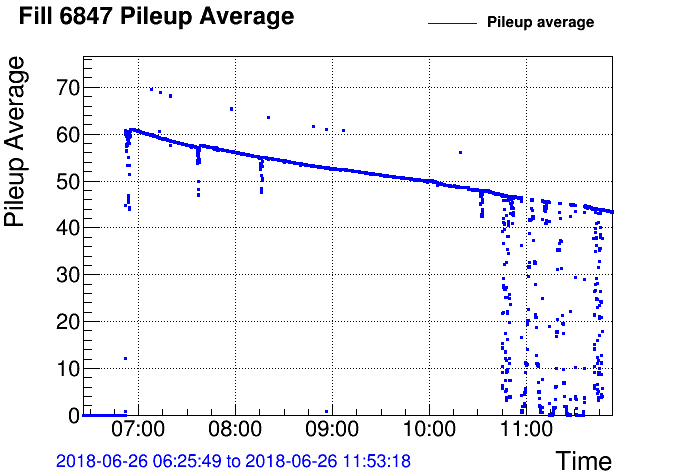
\includegraphics[width=0.55\linewidth]{plots/fill_6847_pileup_avg.png}
    \caption{
      Pileup profile for LHC fill 6847. Two pileup scans were performed between 11:00-11:30.
      \label{fig:fillpu6847}
    }
  \end{center}
\end{figure}

\begin{figure}[hbt]
  \begin{center}
    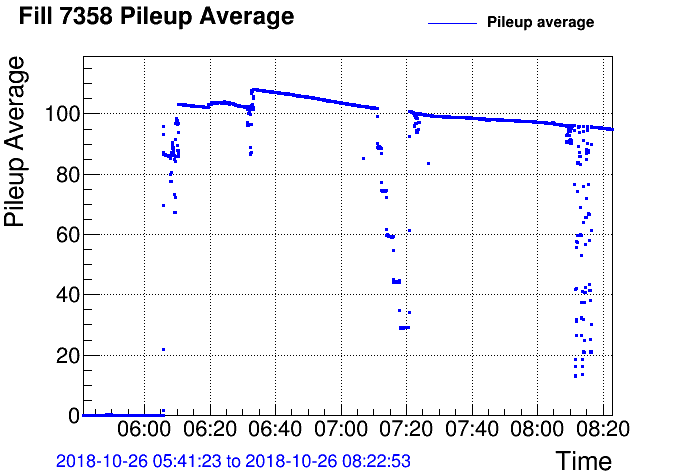
\includegraphics[width=0.55\linewidth]{plots/fill_7358_pileup_avg.png}
    \caption{
      Pileup profile for LHC fill 7358. A pileup scan was performed between  07:10-07:20.
      \label{fig:fillpu7358}
    }
  \end{center}
\end{figure}

\clearpage
\begin{figure}[hbt]
  \begin{center}

    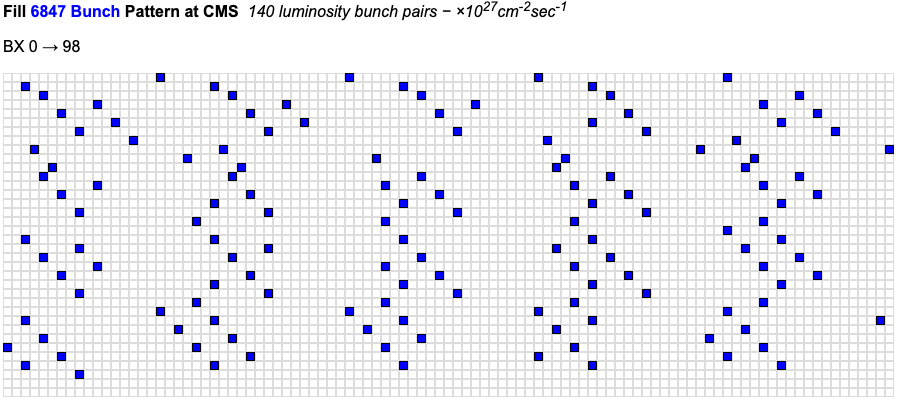
\includegraphics[width=0.99\linewidth]{plots/fillpattern_6847.png}
    \caption{
      Colliding bunch pattern for LHC fill 6847. 
    \label{fig:fill6847pattern}
    }

    \vspace{12pt}
    
    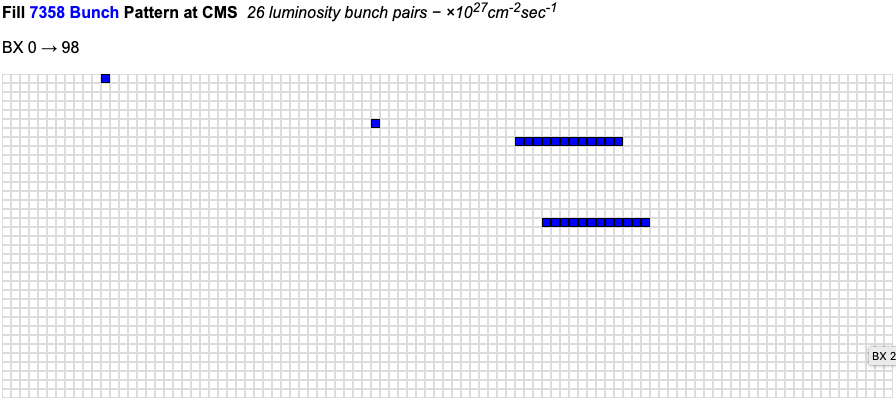
\includegraphics[width=0.99\linewidth]{plots/fillpattern_7358.png}
    \caption{
      Colliding bunch pattern for LHC fill 7358. 
    \label{fig:fill7358pattern}
    }

  \end{center}
\end{figure}


\clearpage
\newpage
\section{Pixel Cluster Counting (PCC) configuration}

\begin{figure}[t]
  \begin{center}
    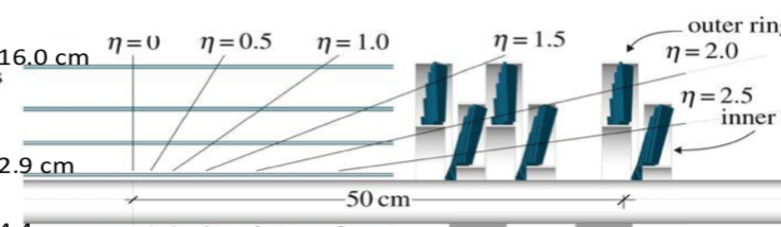
\includegraphics[width=0.9\linewidth]{plots/PixLayout.png}
    \caption{
      Layout of the Phase-1 Pixel detector showing the 4 Barrel layers (0,1,2,3) and 3 Forward disks composed of 2 Panels each. 
    \label{fig:pixellayout}
    }
  \end{center}
\end{figure}


The layout of one quadrant of the Pixel detector used in CMS for  Run II is shown in Figure ~\ref{fig:pixellayout}.
It is composed of a Barrel section with 4 layers and the Forward section each with 3 disks (each with 2 panels) \cite{Collaboration_2008,tracking,pixeldet2017}.
The Pixel sensors are read out by a total of 1856 modules.
A stability study comparing different periods in 2018 was used to exclude a list of modules which showed large variations between periods.
A total of 1387 modules are removed, this veto list can be found in Appendix~\ref{sec:appendix1} and maps per detector section are shown in Figure~\ref{fig:pixelmodvetomap} and Table~\ref{tab:pixveto}.
After the module veto the relative weights of each detector have the values shown in Figure~\ref{fig:pixelweights}.

\begin{table}[hc]
\caption{Number of vetoed modules per Pixel section.}
\label{tab:pixveto}
\begin{center}
\begin{tabular}{l|c|c}
\hline
\multirow{2}{*}{Section} & \multicolumn{2}{c}{$\#$ of Removed modules}  \\
  & $-$Side & $+$Side \\
\hline
BPIX layer 0 & - & - \\
BPIX layer 1 & 108 & 110 \\
BPIX layer 2 & 94  & 168 \\
BPIX layer 3 & 111 & 186 \\
FPIX Panel 0 & 122 & 122 \\
FPIX Panel 1 & 140 & 132 \\
\hline\hline
\end{tabular}
\end{center}
\end{table}


\newpage
\begin{figure}[hbt]
  \begin{center}

    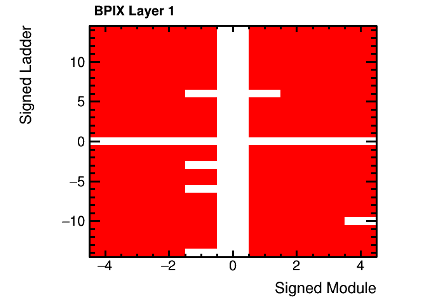
\includegraphics[width=0.45\linewidth]{plots/VetoMap_BPIX1.png}\\
    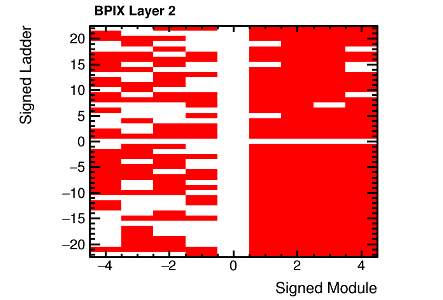
\includegraphics[width=0.45\linewidth]{plots/VetoMap_BPIX2.png}
    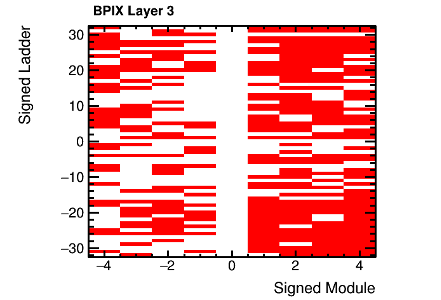
\includegraphics[width=0.45\linewidth]{plots/VetoMap_BPIX3.png}
    \vspace{20pt}
    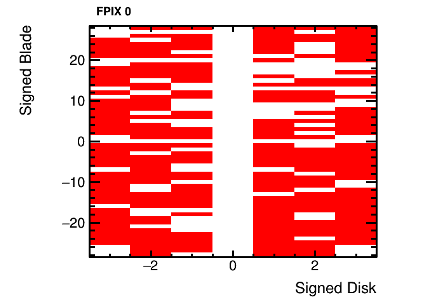
\includegraphics[width=0.45\linewidth]{plots/VetoMap_FPIX0.png}
    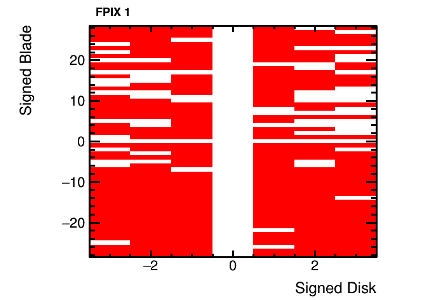
\includegraphics[width=0.45\linewidth]{plots/VetoMap_FPIX1.png}
    \caption{
      Maps of Pixel modules vetoed in the PCC luminosity computation. The veto list corresponds to the study performed using 2018 data including Run D period.
    \label{fig:pixelmodvetomap}
    }
  \end{center}
\end{figure}



\newpage
\begin{figure}[hc]
  \begin{center}
    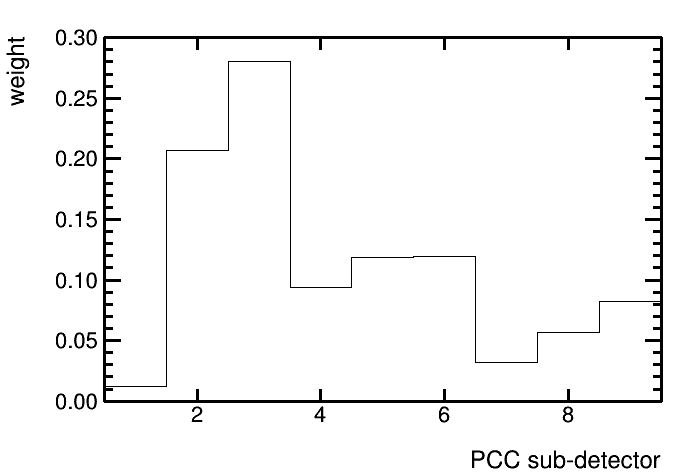
\includegraphics[width=0.7\linewidth]{plots/PCCWeights.png}
    \caption{
      Fraction of total clusters per each part of the Pixel detector. The weights are determined after applying the module veto list.
      Bins 1,2,3 correspond to the BPIX layers, bins 4,5,6 correspond to the FPIX Panel 0 disks (inner), and 7,8,9 to the FPIX Panel 1 disks (outer).
      \label{fig:pixelweights}
    }
  \end{center}
\end{figure}

\clearpage
\newpage
\section{Data sets and visible cross-sections}

For the PCC luminosity determination two types of data-sets are processed, Random trigger data for determination of ``afterglow'' corrections using the noise observed in non-colliding bunches, and ZeroBias data for the cluster counting in colliding bunches.
The data samples are stored in ALCARECO format in the CERN EOS system in the paths shown in Table~\ref{tab:datapaths}.

Additional data is needed to obtain the corresponding luminosity for the HF, PLT, and BCM luminometers.
For these detectors the BRIL data acquisition system (\emph{BRIL-DAQ}) is used and the data is stored in HD5 file format in special machines at Point 5 (\emph{brildev}).
The data samples used are shown in the Table~\ref{tab:datapathsbrildev}.
For these luminometers no additional corrections are applied, except for the HFOC residual afterglow.

The HF luminometer data in the hd5 files does not include final afterglow corrections for the HFOC algorithm.
These corrections have been obtained separately in ROOT histogram format from the Princeton group, and are currently stored in the following public directory:\\
\emph{/afs/cern.ch/user/j/jingyu/public/LUMI/for\_jose/}

The visible cross-sections used to normalize the data from each luminometer are listed in Table~\ref{tab:crossections}.
The values used for each luminometer differ from the ones listed in the 2018 PAS due to corrections which are needed for each detector as described in the table.




\clearpage
\begin{table}[h]
  \caption{Paths to the data used for the PCC luminosity determination (ZeroBias) and afterglow corrections (Random).
  The data paths are relative to the CERN eos system: $/eos/cms/store/$
  }
  \label{tab:datapaths}
  \footnotesize
  \begin{tabular}{l}
    \hline\hline
    Fill 6847:\\
data/Run2018B/AlCaLumiPixels/ALCARECO/AlCaPCCRandom-PromptReco-v2/000/318/675/\\ %00000/1E77B884-FF7A-E811-803C-FA163E76D066.root \\
data/Run2018B/AlCaLumiPixels0/ALCARECO/AlCaPCCZeroBias-PromptReco-v2/000/318/675/\\ %00000/9A8628CC-DF7A-E811-A671-FA163EDE4F34.root \\
data/Run2018B/AlCaLumiPixels1/ALCARECO/AlCaPCCZeroBias-PromptReco-v2/000/318/675/\\ %00000/16F2BA8F-D97A-E811-9385-FA163EA487EB.root \\
data/Run2018B/AlCaLumiPixels2/ALCARECO/AlCaPCCZeroBias-PromptReco-v2/000/318/675/\\ %00000/0677196F-D67A-E811-8E4E-FA163EF568AC.root \\
data/Run2018B/AlCaLumiPixels3/ALCARECO/AlCaPCCZeroBias-PromptReco-v2/000/318/675/\\ %00000/D8813469-D57A-E811-84C8-FA163E18DCD1.root \\
data/Run2018B/AlCaLumiPixels4/ALCARECO/AlCaPCCZeroBias-PromptReco-v2/000/318/675/\\ %00000/DECE9555-FD7A-E811-A11F-FA163E5B62DF.root \\
data/Run2018B/AlCaLumiPixels5/ALCARECO/AlCaPCCZeroBias-PromptReco-v2/000/318/675/\\ %00000/BA53B331-EE7A-E811-8AC2-02163E019EC5.root \\
data/Run2018B/AlCaLumiPixels6/ALCARECO/AlCaPCCZeroBias-PromptReco-v2/000/318/675/\\ %00000/4E162320-E47A-E811-B5EA-FA163EB7AC61.root \\
data/Run2018B/AlCaLumiPixels7/ALCARECO/AlCaPCCZeroBias-PromptReco-v2/000/318/675/\\ %00000/22A4C262-E17A-E811-AFEF-FA163E336245.root \\
data/Run2018B/AlCaLumiPixels8/ALCARECO/AlCaPCCZeroBias-PromptReco-v2/000/318/675/\\ %00000/F69D7D47-E77A-E811-9C74-FA163E163082.root \\
data/Run2018B/AlCaLumiPixels9/ALCARECO/AlCaPCCZeroBias-PromptReco-v2/000/318/675/\\ %00000/680CF7EB-D47A-E811-BAFB-FA163EA487EB.root \\
\hline
    Fill 7358:\\
express/Run2018E/StreamALCALUMIPIXELSEXPRESS/ALCARECO/AlCaPCCRandom-Express-v1/000/325/309/\\ %00000/4C63A580-3BA2-0D4E-A447-E5A980883D1E.root \\
data/Run2018E/AlCaLumiPixels1/ALCARECO/AlCaPCCZeroBias-PromptReco-v1/000/325/309/\\ %00000/3993D954-4C5C-2247-8935-A8D6019151B7.root \\
data/Run2018E/AlCaLumiPixels2/ALCARECO/AlCaPCCZeroBias-PromptReco-v1/000/325/309/\\ %00000/E56486D8-15C1-6E47-BB5B-C798DC7B35E5.root \\
data/Run2018E/AlCaLumiPixels3/ALCARECO/AlCaPCCZeroBias-PromptReco-v1/000/325/309/\\ %00000/7136F0DC-3A4B-4445-8AB4-9EA9D9BE16F6.root \\
data/Run2018E/AlCaLumiPixels4/ALCARECO/AlCaPCCZeroBias-PromptReco-v1/000/325/309/\\ %00000/B0920DA1-D6B5-1545-BA56-7597EB33FD47.root \\
data/Run2018E/AlCaLumiPixels5/ALCARECO/AlCaPCCZeroBias-PromptReco-v1/000/325/309/\\ %00000/96C74CCD-682A-5D47-9AC8-BE229BD27DA3.root \\
data/Run2018E/AlCaLumiPixels6/ALCARECO/AlCaPCCZeroBias-PromptReco-v1/000/325/309/\\ %00000/415CC662-DB7D-F74F-9FB9-AB878EF770C5.root \\
data/Run2018E/AlCaLumiPixels7/ALCARECO/AlCaPCCZeroBias-PromptReco-v1/000/325/309/\\ %00000/A4711D16-DB69-7447-93FF-4CA53B476927.root \\
data/Run2018E/AlCaLumiPixels8/ALCARECO/AlCaPCCZeroBias-PromptReco-v1/000/325/309/\\ %00000/CC2437DB-E2CD-444D-832A-BAF3C7592C21.root \\
data/Run2018E/AlCaLumiPixels9/ALCARECO/AlCaPCCZeroBias-PromptReco-v1/000/325/309/\\ %00000/E7DA9BE1-28F3-3A40-98A9-A22761530735.root \\
\hline\hline
  \end{tabular}
\end{table}

\vspace{24pt}
\begin{table}[h]
\begin{center}
\caption{Paths to the data used for the HF, BCM, and PLT luminometers. This data is stored in the \emph{brildev} system at Point 5.}
  \label{tab:datapathsbrildev}
 % \footnotesize
  \begin{tabular}{c|l}
    \hline\hline
Fill & Data Path \\
6847 &  /brildata/vdmdata18/6847\_1806261047\_1806261133.hd5 \\
7358 & /brildata/vdmdata18/7358\_1810260704\_1810260726.hd5  \\
    \hline\hline
  \end{tabular}
\end{center}
\end{table}


\vspace{24pt}
\begin{table}[h]
  \caption{Visible cross-sections used for each luminometer in this analysis. The differences with respect to the values in the 2018 PAS \cite{CMS-PAS-LUM-18-002} are described in the third column.}
  \label{tab:crossections}
    \begin{tabular}{l|c|c}
      \hline
      Luminometer & $\sigma_{vis}$ & Difference w.r.t \cite{CMS-PAS-LUM-18-002}\\
      \hline
      PCC   &  3140  $mb$     & This value corresponds to a tighter module veto list. \\
      HFOC  &  797.5 $\mu b$  & This value is further corrected by 0.987 for radiation damage in Fill 7358. \\
      BCM1F &  203.2 $\mu b$  &   \\
      PLT   &  305   $\mu b$  & Corrected using emmittance scan data. \\
      \hline\hline
    \end{tabular}
\end{table}

\clearpage
\newpage
\section{Afterglow corrections}

The PCC luminosity determination requires corrections for ``afterglow'' effects, noise induced in bunch crossings following colliding bunch crossings.
Two corrections have been previously developed: Type-1 refers to a spill over into the bunch crossing immediately following an active bunch crossing due to charge residuals in the pixel sensors, the second Type-2 refers to exponentially decaying noise created by activated material.
The models for both corrections are normalized using data from empty bunch crossings recorded with \random\ triggers.
The corrections are stored in the CMS Conditions Database during the Prompt Calibration Loop (PCL).
The PCC values obtained from the \zerobias\ trigger data are then corrected in an offline analysis.
Similar afterglow corrections are obtained for HFOC.

The afterglow corrections are normally calculated for an integrated range of lumi sections to improve the statistical precision, for PCC every 50 LS while for HFOC every 20. In this study the PCC corrections were determined privately every 10 LS to capture variations during $\mu$-scans.
Example corrections (Type-1 and Type-2 combined) are showin in Figure~\ref{fig:afterglow}.
For fill 6847 the corrections have values of 1.0 due to the single bunch pattern.

\begin{figure}[t]
  \begin{center}
    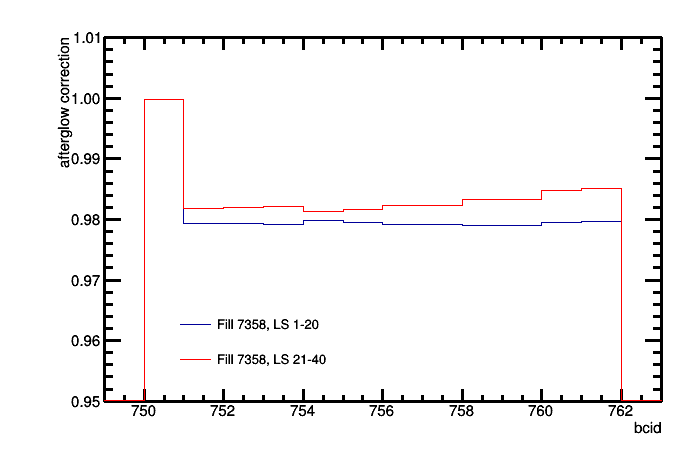
\includegraphics[width=0.47\linewidth]{plots/HFAfterglowCorr.png}
    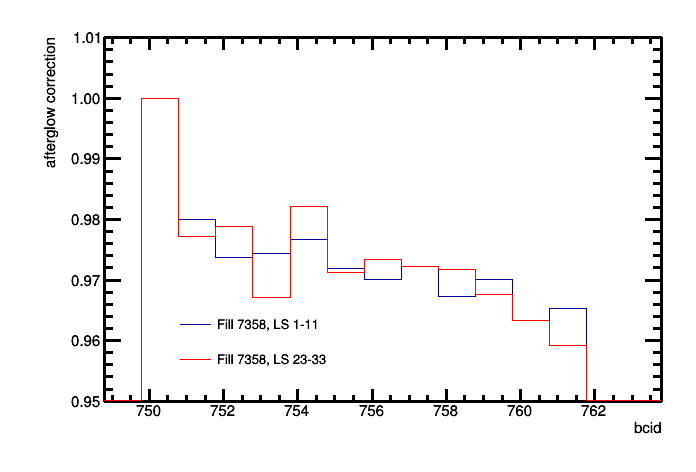
\includegraphics[width=0.47\linewidth]{plots/PCCAfterglowCorr.png}
    \caption{
      Afterglow corrections for HFOC (left) and PCC (right) as a function of bcid for one bunch train in fill 7358.
      The different curves show the difference between low and high pileup lumisections.
    \label{fig:afterglow}
    }
  \end{center}
\end{figure}


\clearpage
\newpage
\section{Time selections}

The luminometer data corresponding to the $\mu$-scans is selected by applying selections on the time stamps.
The selections remove luminosity values when the LHC beam conditions are in transition.
The time selections are best determined from one of the luminometers read by the BRIL-DAQ as the temporal granularity has ``nibble'' resolution ($\sim$2s), while the PCC luminosity values are determined every lumi section ($\sim$23s).

Figure~\ref{fig:lumivstime} shows the luminosity vs. time for the HFOC luminometer and the transition time stamps that were determined from these data.
The absolute time stamp values in seconds are the following:
\begin{itemize}
\item Fill 6847 : 1530010610, 1530010615, 1530010670, 1530010721, 1530010772, 1530010824, 1530010875, 1530010926, 1530010978, 1530011031, 1530011082, 1530011133, 1530011184, 1530011235, 1530011287, 1530011339, 1530011393, 1530011441, 1530011489, 1530011537, 1530011585, 1530011633, 1530011681, 1530011729, 1530011761, 1530011811, 1530011863, 1530011914, 1530011966, 1530012019, 1530012070, 1530012122, 1530012173, 1530012225, 1530012277, 1530012328, 1530011400
\item Fill 7358 : 1540537829, 1540537864, 1540537940, 1540538037, 1540538158, 1540538277, 1540538446, 1540538429
\end{itemize}

All data  within 24 seconds of these transitions times are excluded from the analysis, in the case of PCC the luminosity sections with time stamps in these windows are removed.
The data for luminometers with nibble granualurity (HFOC, PLT, BCM) are then averaged within the corresponding  lumisections for comparison with PCC. 
The PCC and HFOC luminosity values per lumisection before and after the time selections are shown in Figure~\ref{fig:lumivsls}.


\begin{figure}[t]
  \begin{center}
    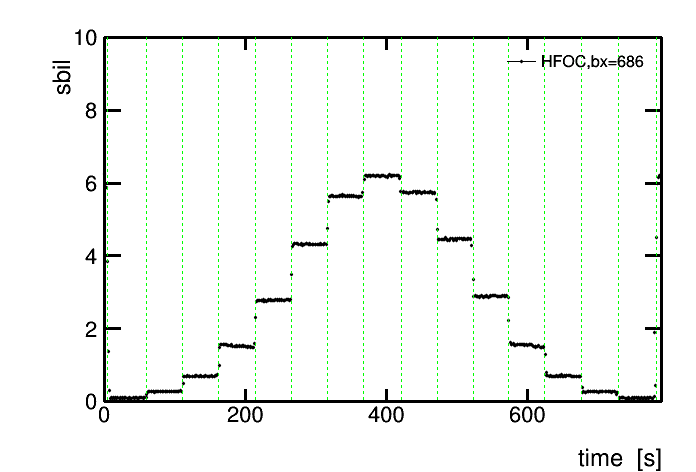
\includegraphics[width=0.47\linewidth]{plots/plot_lumi_vstime_6847.png}
    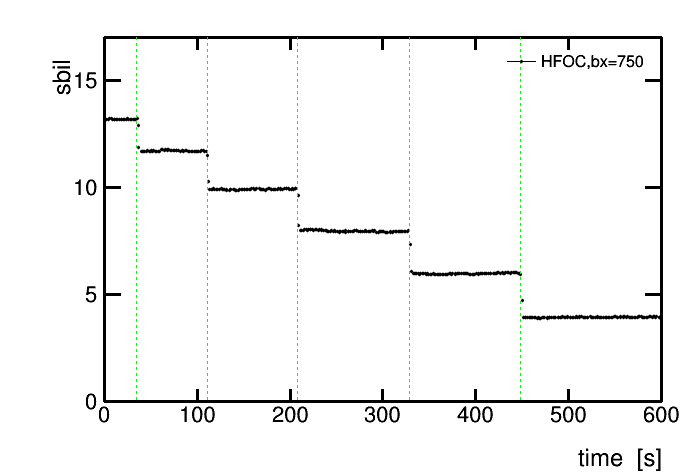
\includegraphics[width=0.47\linewidth]{plots/plot_lumi_vstime_7358.png}
    \caption{
      SBIL data for the HFOC covering the time range of one $\mu$-scan in Fill 6847 (left) and Fill 7358 (right). The vertical lines mark the time stamps determined from this data where the LHC beam parameters are changed.
    \label{fig:lumivstime}
    }
  \end{center}
\end{figure}


\newpage

\begin{figure}[t]
  \begin{center}
    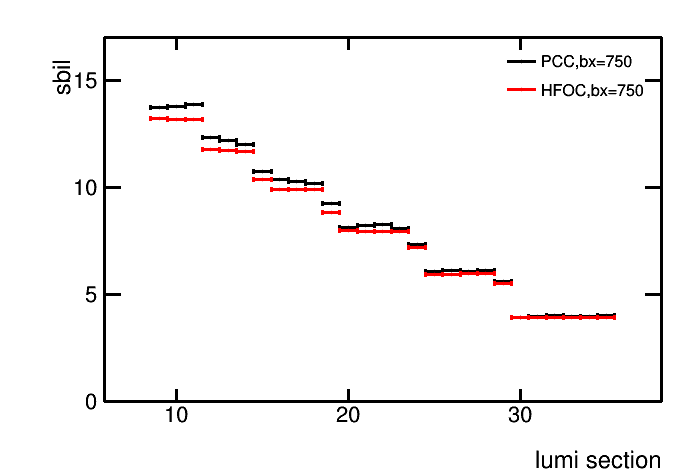
\includegraphics[width=0.6\linewidth]{plots/plot_lumi_vsls_7358_before.png}
    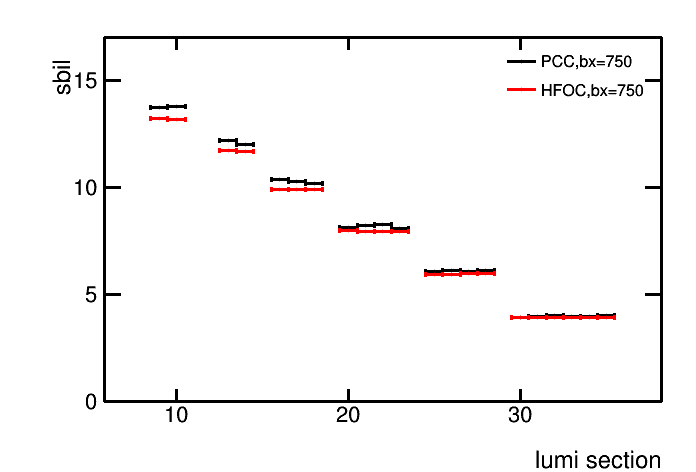
\includegraphics[width=0.6\linewidth]{plots/plot_lumi_vsls_7358_after.png}
    \caption{
    PCC and HFOC single bunch instantenous luminosity (SBIL) for one bunch crossing in Fill 7358 before (top) and after (bottom) applying the time selections.
    \label{fig:lumivsls}
    }
  \end{center}
\end{figure}

\clearpage
\newpage
\section{Relative linearity determination}

The determination of the relative linearity between two luminometers requires fitting for the slope in the ratio of the SBIL values as a function of SBIL.
In the nominal comparison the HFOC is chosen as a reference luminometer due to its good statistical precision and stability.
The linearity is studied for individual bunch crossings after the corrections and selections described before.

In order to assign an uncertainty on the PCC/HFOC ratio at a given SBIL, ratio values computed for individual lumisections are grouped and averaged if their reference SBIL values are within 0.5.
The uncertainty is assigned as the standard deviation of the ratios used in the average.
Figure~\ref{fig:sbilratiomethod} illustrates the method, the resulting graph is fit using a linear function.


In Figures~\ref{fig:sbilratios6847} and \ref{fig:sbilratios7358} the linearity fits are shown for the single and leading bunches in fill 6847 and 7358.
Figures~\ref{fig:sbilratiosresults6847} and \ref{fig:sbilratiosresults7358} summarize  the fit parameter results.


Figure~\ref{fig:sbilratios_dets} compares the correlations and ratios between different luminometers for fill 7358.

\begin{figure}[t]
  \begin{center}
    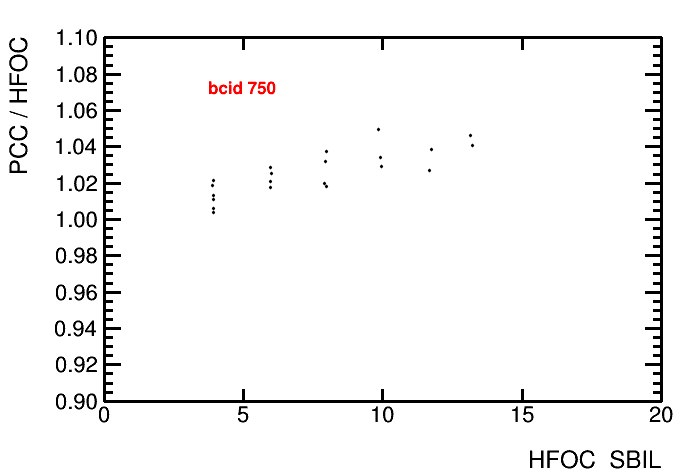
\includegraphics[width=0.47\linewidth]{plots/plot_det_linearity_perbx_pcc_7358_750_scatter.png}
    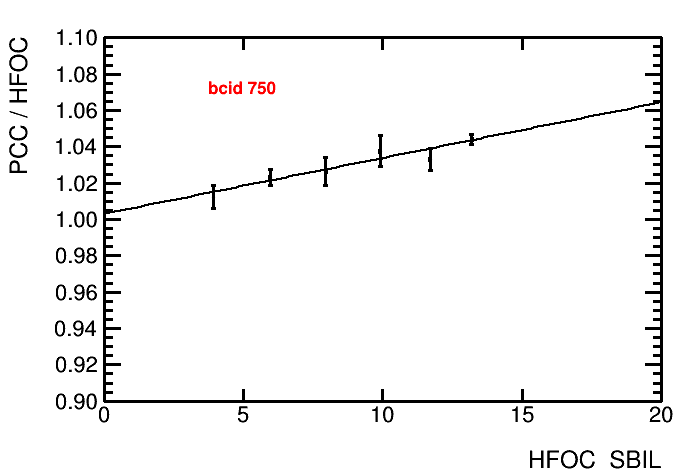
\includegraphics[width=0.47\linewidth]{plots/plot_det_linearity_perbx_pcc_7358_750_avg.png}
    \caption{
      PCC / HFOC  SBIL ratios as a function of HFOC SBIL for one bunch crossing in Fill 7358.
      The graphs illustrate the method for determining the average ratio at a given SBIL value as described in the text.
    \label{fig:sbilratiomethod}
    }
  \end{center}
\end{figure}

\clearpage
\begin{figure}[t]
  \begin{center}
    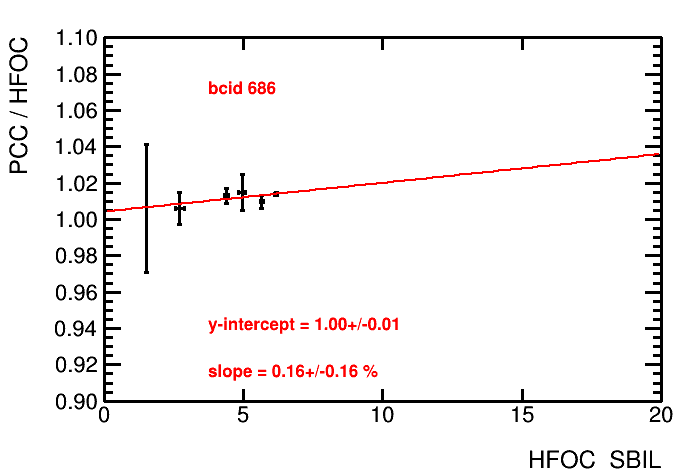
\includegraphics[width=0.47\linewidth]{plots/sbilratios_singles/plot_det_linearity_perbx_pcc_6847_686.png}
    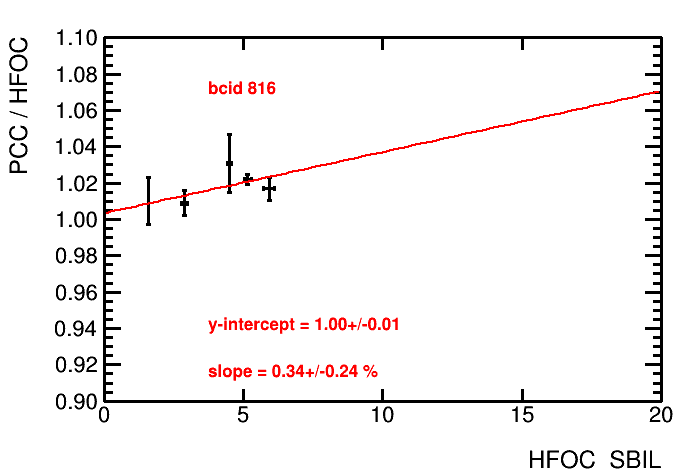
\includegraphics[width=0.47\linewidth]{plots/sbilratios_singles/plot_det_linearity_perbx_pcc_6847_816.png}
    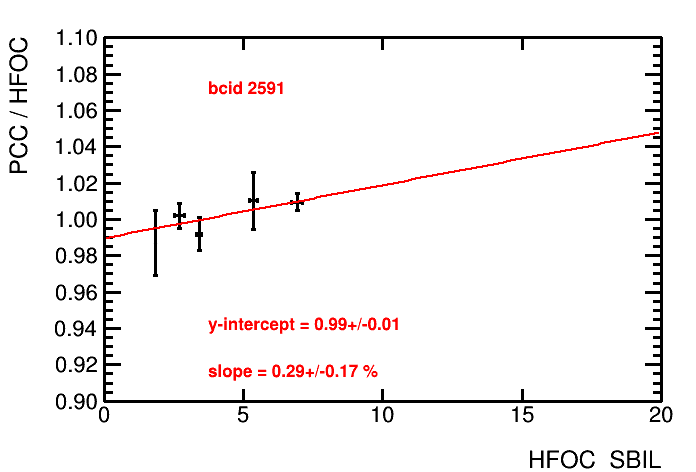
\includegraphics[width=0.47\linewidth]{plots/sbilratios_singles/plot_det_linearity_perbx_pcc_6847_2591.png}
    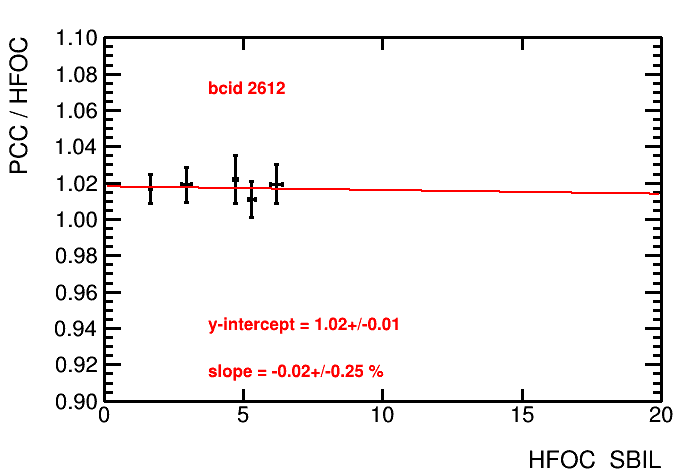
\includegraphics[width=0.47\linewidth]{plots/sbilratios_singles/plot_det_linearity_perbx_pcc_6847_2612.png}
    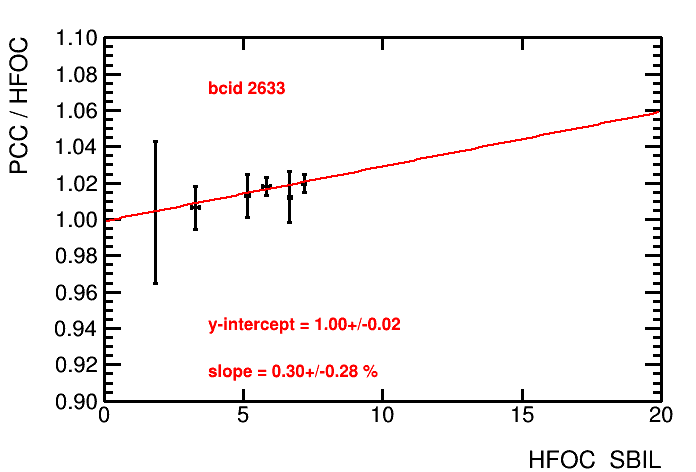
\includegraphics[width=0.47\linewidth]{plots/sbilratios_singles/plot_det_linearity_perbx_pcc_6847_2633.png}
    \caption{
      Ratio of PCC over HFOC single bunch instantenous luminosity (SBIL) as a function of SBIL for the 5 high statistics bunches in Fill 6847.
      The points and error bars are determined as described in the text.
    \label{fig:sbilratios6847}
    }
  \end{center}
\end{figure}

\clearpage
\begin{figure}[t]
  \begin{center}
    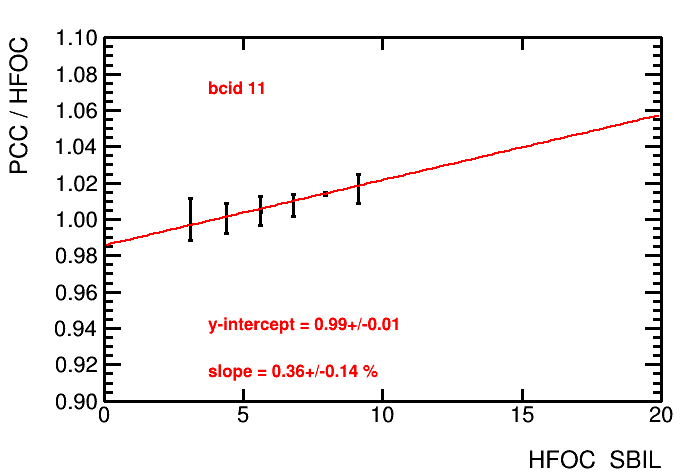
\includegraphics[width=0.47\linewidth]{plots/sbilratios_singles/plot_det_linearity_perbx_pcc_7358_11.png}
    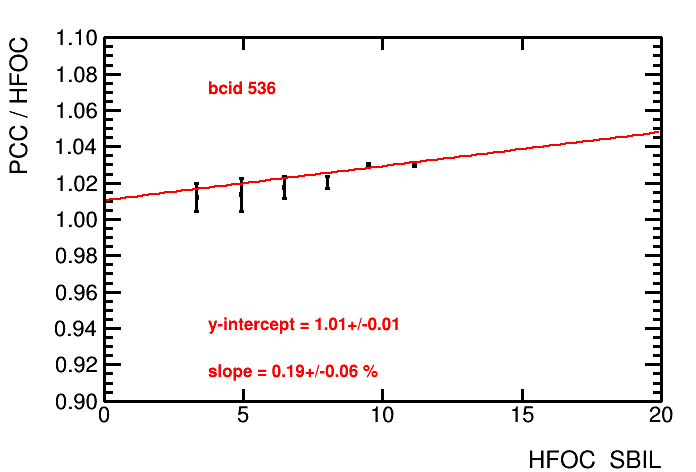
\includegraphics[width=0.47\linewidth]{plots/sbilratios_singles/plot_det_linearity_perbx_pcc_7358_536.png}
    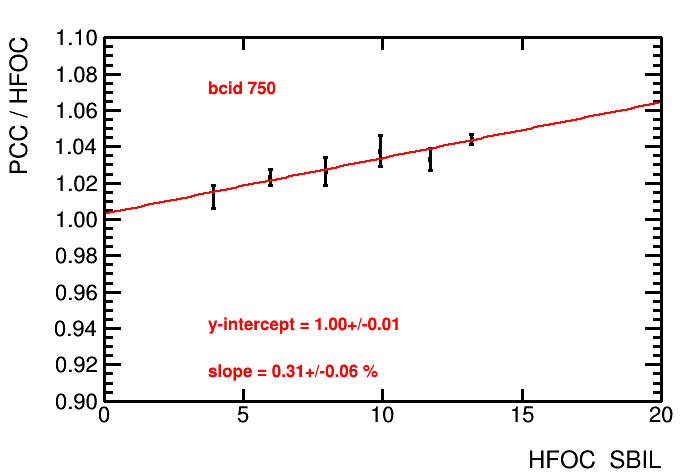
\includegraphics[width=0.47\linewidth]{plots/sbilratios_singles/plot_det_linearity_perbx_pcc_7358_750.png}
    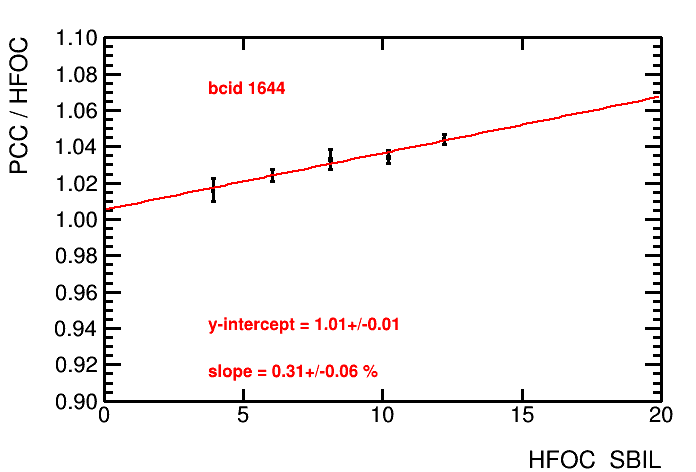
\includegraphics[width=0.47\linewidth]{plots/sbilratios_singles/plot_det_linearity_perbx_pcc_7358_1644.png}
    \caption{
      Ratio of PCC over HFOC single bunch instantenous luminosity (SBIL) as a function of SBIL for the 2 solo and 2 leading  bunches in Fill 7358.
      The points and error bars are determined as described in the text.
      \label{fig:sbilratios7358}
    }
  \end{center}
\end{figure}

\clearpage
\begin{figure}[t]
  \begin{center}
    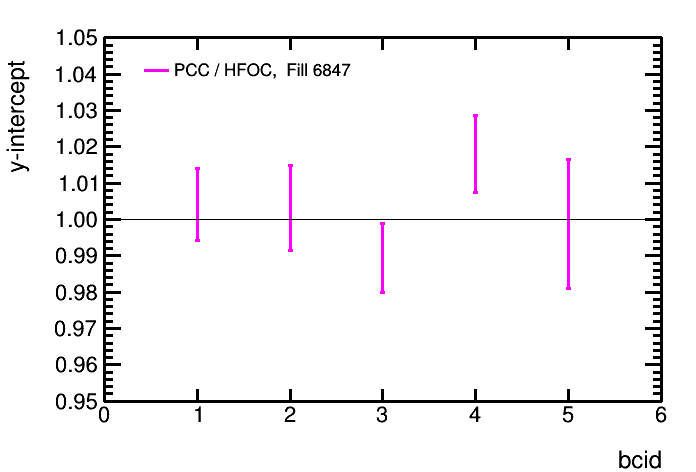
\includegraphics[width=0.47\linewidth]{plots/sbilratios_singles/plot_det_linearity_perbx_y0_6847.png}
    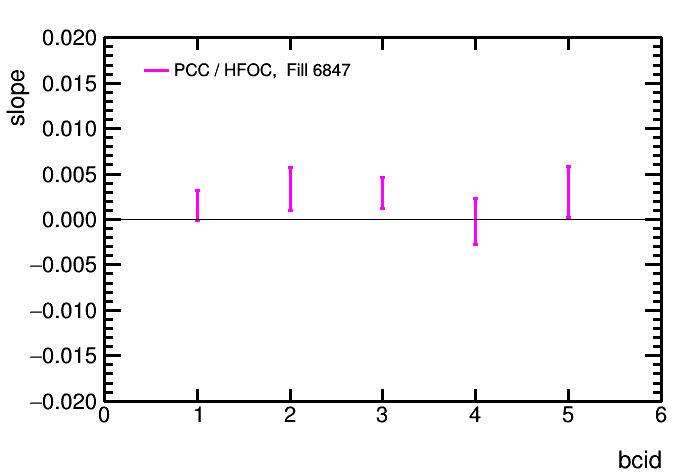
\includegraphics[width=0.47\linewidth]{plots/sbilratios_singles/plot_det_linearity_perbx_slope_6847.png}
    \caption{
      y-intercept (left) and slope (right) for the linear fits to the ratios of PCC/HFOC v.s. SBIL for the 5 high statistics bunches in Fill 6847.
      \label{fig:sbilratiosresults6847}
    }
  \end{center}
\end{figure}

\begin{figure}[t]
  \begin{center}
    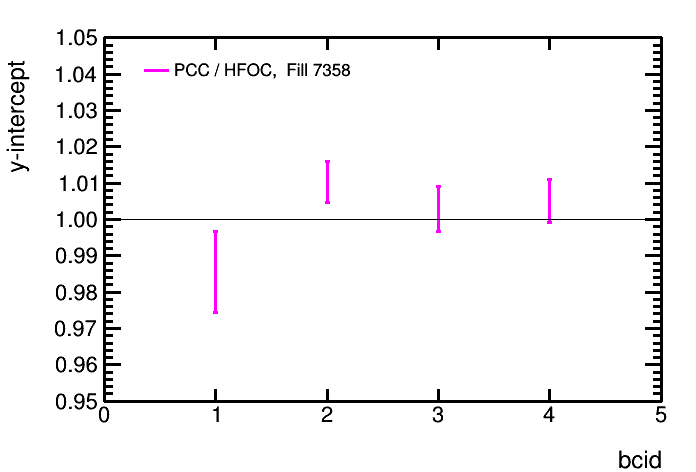
\includegraphics[width=0.47\linewidth]{plots/sbilratios_singles/plot_det_linearity_perbx_y0_7358.png}
    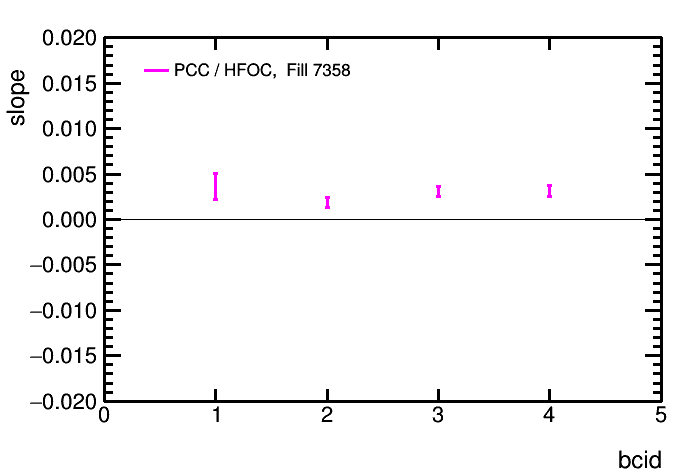
\includegraphics[width=0.47\linewidth]{plots/sbilratios_singles/plot_det_linearity_perbx_slope_7358.png}
    \caption{
      y-intercept (left) and slope (right) for the linear fits to the ratios of PCC/HFOC v.s. SBIL for the 2 solo and 2 leading  bunches in Fill 7358.
      \label{fig:sbilratiosresults7358}
    }
  \end{center}
\end{figure}


\clearpage
\begin{figure}[t]
  \begin{center}
    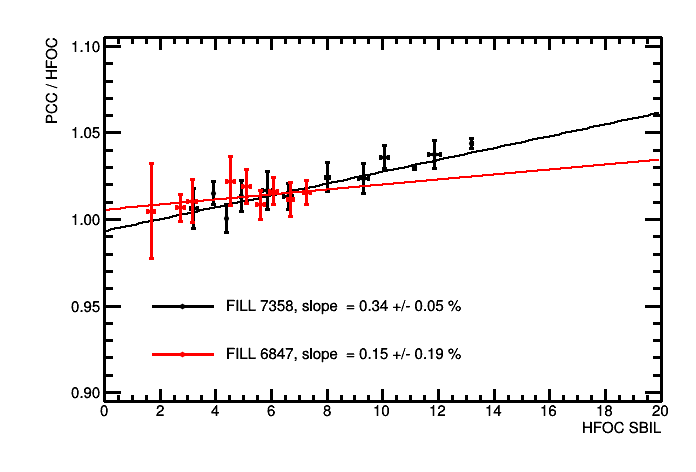
\includegraphics[width=0.7\linewidth]{plots/sbilratios_singles_combined/compareFills_graph_fillstogether.png}
    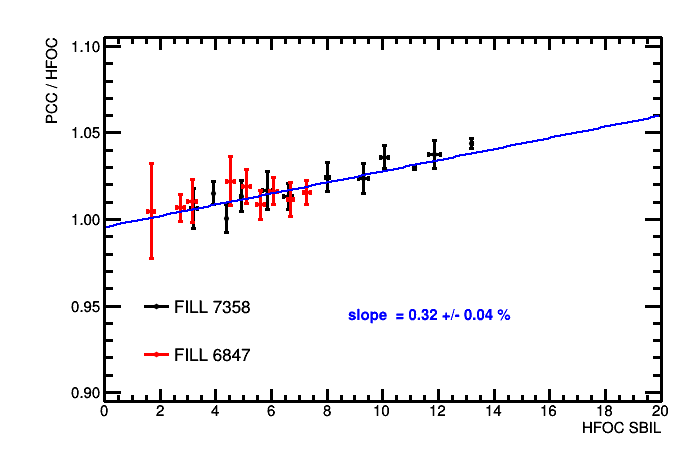
\includegraphics[width=0.7\linewidth]{plots/sbilratios_singles_combined/compareFills_graph_fillstogether_onefit.png}
    \caption{
      Comparison of the ratio of PCC / HFOC after combining all leading and solo bunches in fills 6847 and 7358.
      The data points and uncertainties are determined as described in the text.
      The fills are fit separately (top) and together (bottom).
      \label{fig:sbilratiosresultscombined}
    }
  \end{center}
\end{figure}


\clearpage
\begin{figure}[t]
  \begin{center}
    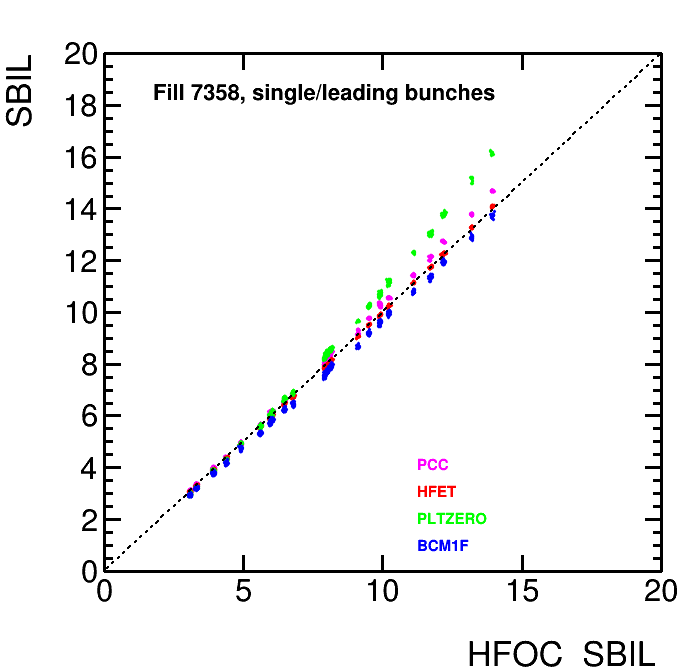
\includegraphics[width=0.47\linewidth]{plots/sbilratios_singles/plot_linearity_det_correlation.png}
    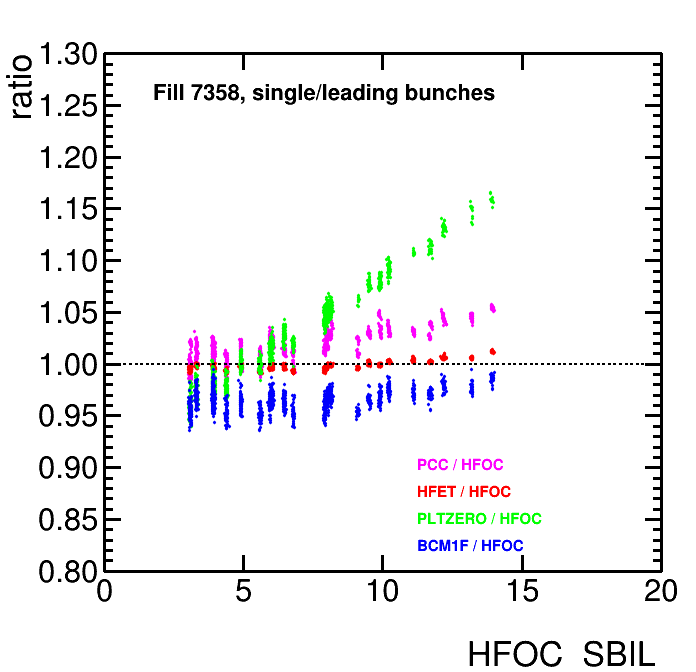
\includegraphics[width=0.47\linewidth]{plots/sbilratios_singles/plot_linearity_det_correlation_ratio.png}
    \caption{
      Correlations (left) and ratios (right) of the SBIL values between different luminometers in Fill 7358.
    \label{fig:sbilratios_dets}
    }
  \end{center}
\end{figure}

\clearpage
\newpage
\section{Train effects}
The dependence of the linearity fit results as a function of  the bunch crossing in the trains is shown in Figures~\ref{fig:fill7358trainresults}.
A systematic drop in the slope is observed as the colliding bunch is farther from the leading bunch.

A check was performed to know if this trend may be caused by the afterglow corrections  as shown in Appendix~\ref{sec:appendix2} where the PCC and HFOC afterglow corrections are removed, however the change in the trend is small.

Comparisons to other luminometers show a similar systematic trend for HFET and BCM1F (Figures~\ref{fig:fill7358trainslope_hfet} and \ref{fig:fill7358trainslope_bcm}).
In the case of PLT (Figure~\ref{fig:fill7358trainslope_plt}) the trend is different and a strong negative slope is obtained for the leading bunch.

The effect was further studied by reprocessing the PCC data while modifying the module veto list to select different parts of the Pixel detector, these results are shown in Figure~\ref{fig:fill7358trainslope_pccparts}.
In these graphs it is observed that BPIX layer 1, FPIX Panel 1 all disks, and FPIX Panel 2 disks 1 show the trend, while the remaining parts are more stable.

\begin{figure}[t]
  \begin{center}
    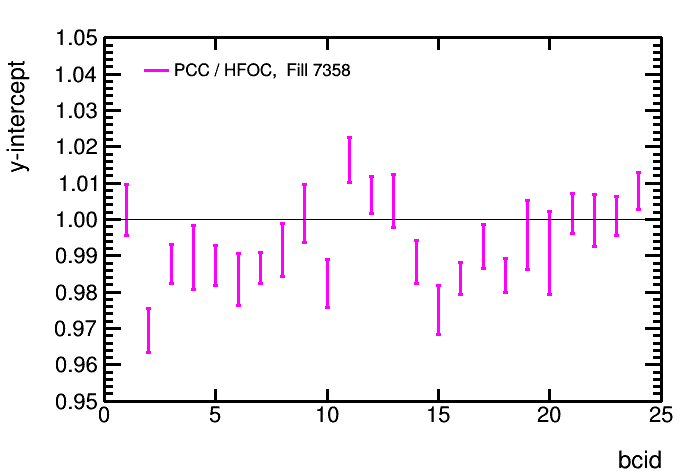
\includegraphics[width=0.47\linewidth]{plots/sbilratios_trains_Fill7358/plot_det_linearity_perbx_y0_7358.png}
    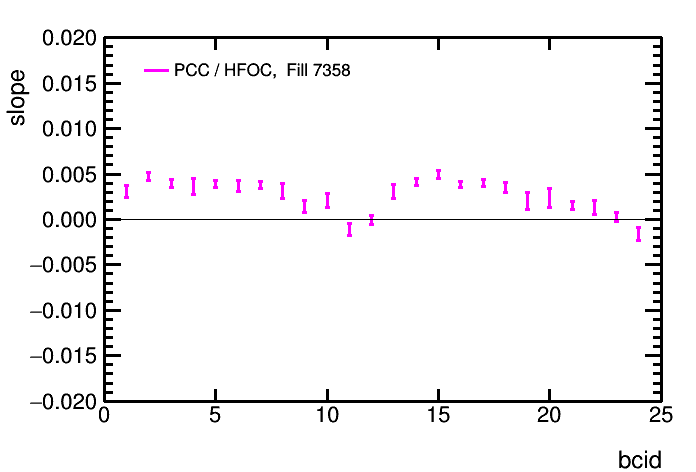
\includegraphics[width=0.47\linewidth]{plots/sbilratios_trains_Fill7358/plot_det_linearity_perbx_slope_7358.png}
    \caption{
      y-intercept and slope values obtained from the linearity fits for the 24 bunches in the two trains of Fill 7358.
      \label{fig:fill7358trainresults}
    }
  \end{center}
\end{figure}



\clearpage
\begin{figure}[t]
  \begin{center}
    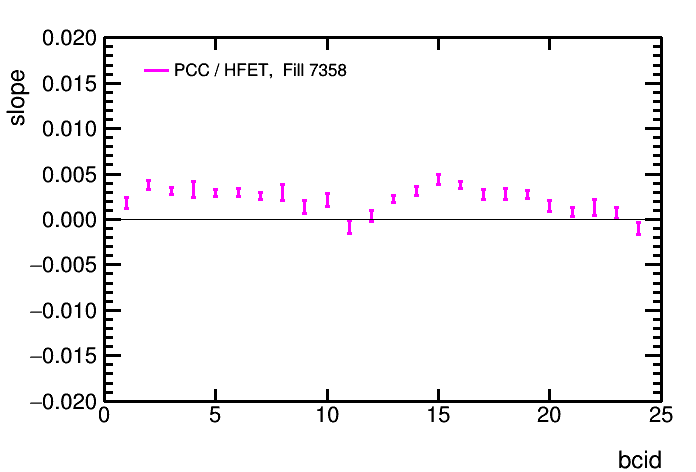
\includegraphics[width=0.47\linewidth]{plots/sbilratios_trains_Fill7358/plot_det_linearity_perbx_slope_7358_hfet.png}
    \caption{
      Slope values obtained from the linearity fits for the 24 bunches in the two trains of Fill 7358, in this plot the PCC is compared to the HFET luminometer.
      \label{fig:fill7358trainslope_hfet}
    }
  \end{center}
\end{figure}

\begin{figure}[t]
  \begin{center}
    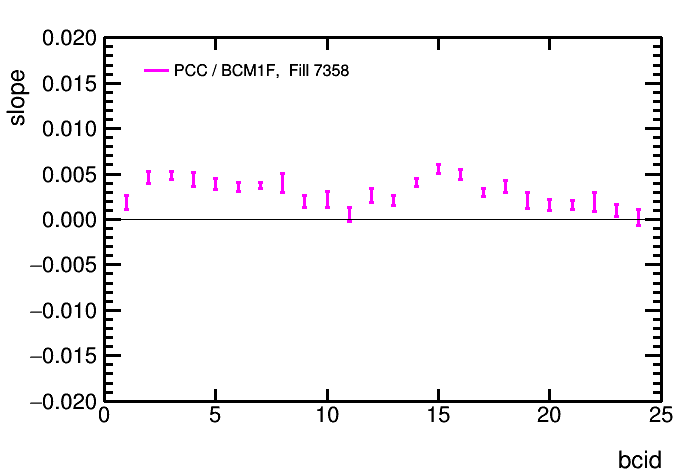
\includegraphics[width=0.47\linewidth]{plots/sbilratios_trains_Fill7358/plot_det_linearity_perbx_slope_7358_bcm.png}
    \caption{
      Slope values obtained from the linearity fits for the 24 bunches in the two trains of Fill 7358, in this plot the PCC is compared to the BCM1F luminometer.
      \label{fig:fill7358trainslope_bcm}
    }
  \end{center}
\end{figure}

\begin{figure}[t]
  \begin{center}
    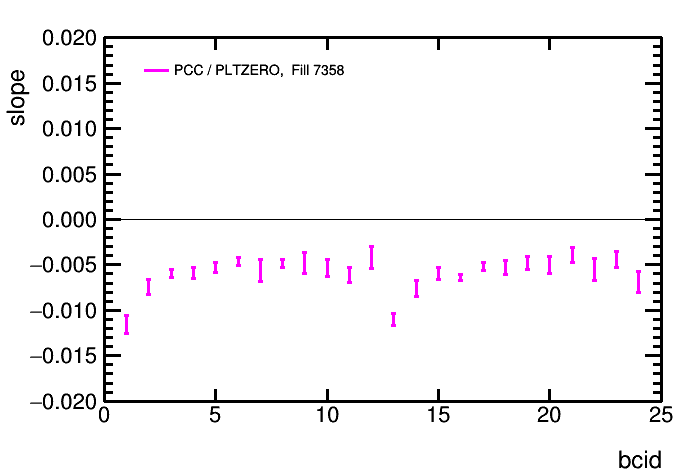
\includegraphics[width=0.47\linewidth]{plots/sbilratios_trains_Fill7358/plot_det_linearity_perbx_slope_7358_plt.png}
    \caption{
      Slope values obtained from the linearity fits for the 24 bunches in the two trains of Fill 7358, in this plot the PCC is compared to the PLTZERO luminometer.
      \label{fig:fill7358trainslope_plt}
    }
  \end{center}
\end{figure}


\clearpage
\begin{figure}[t]
  \begin{center}
    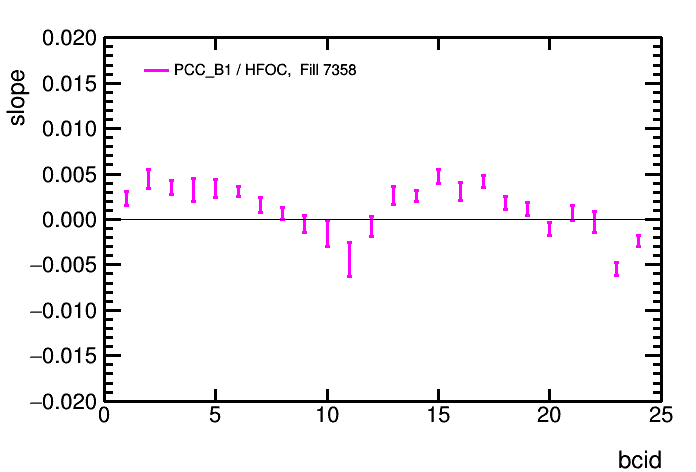
\includegraphics[width=0.32\linewidth]{plots/sbilratios_trains_Fill7358/plot_det_linearity_perbx_slope_7358_B1.png}
    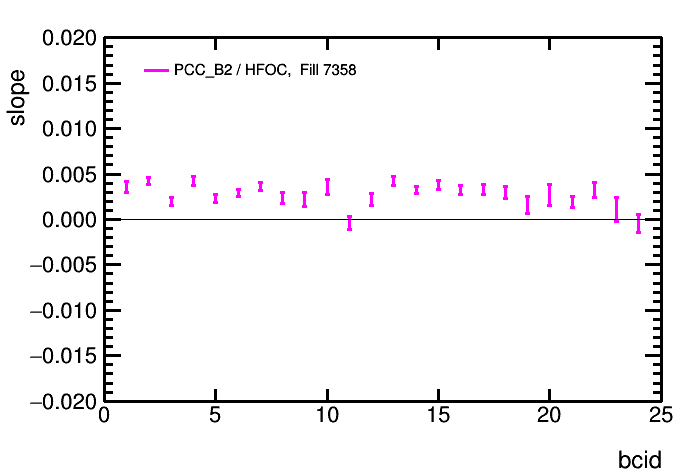
\includegraphics[width=0.32\linewidth]{plots/sbilratios_trains_Fill7358/plot_det_linearity_perbx_slope_7358_B2.png}
    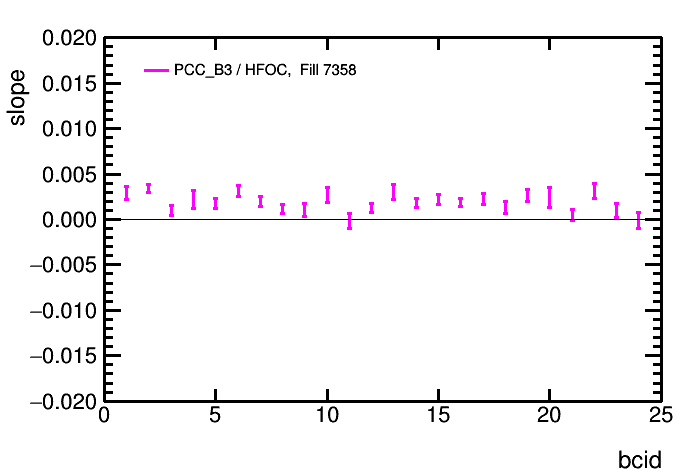
\includegraphics[width=0.32\linewidth]{plots/sbilratios_trains_Fill7358/plot_det_linearity_perbx_slope_7358_B3.png}
    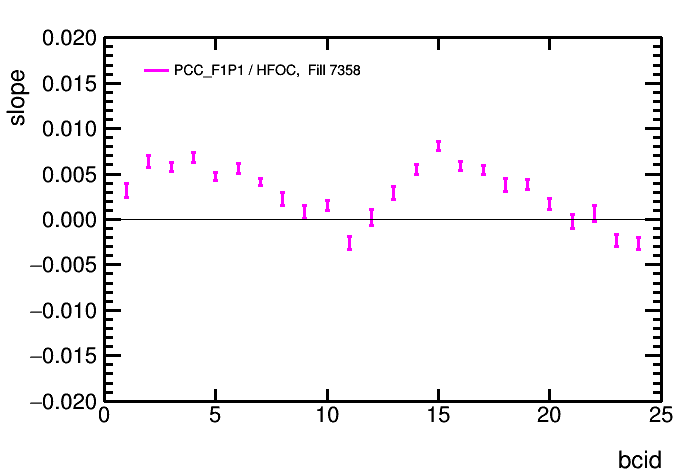
\includegraphics[width=0.32\linewidth]{plots/sbilratios_trains_Fill7358/plot_det_linearity_perbx_slope_7358_F1p1.png}
    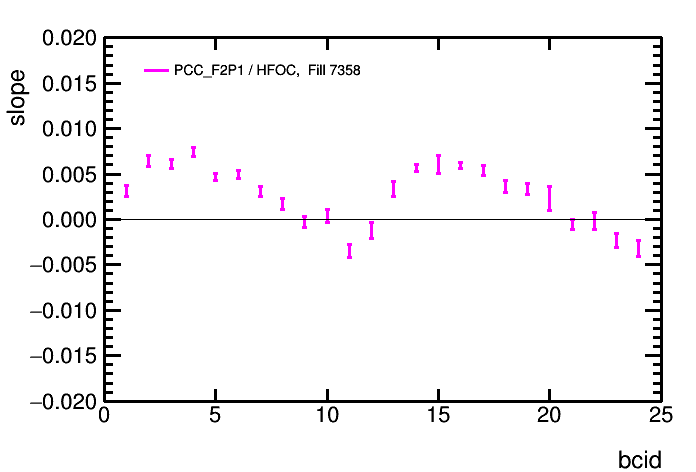
\includegraphics[width=0.32\linewidth]{plots/sbilratios_trains_Fill7358/plot_det_linearity_perbx_slope_7358_F2p1.png}
    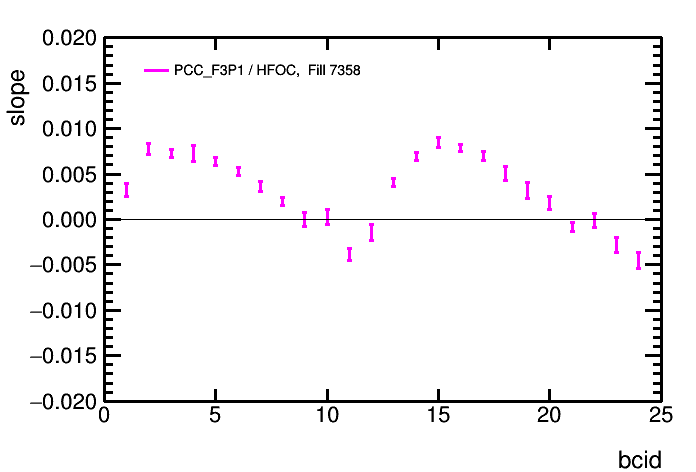
\includegraphics[width=0.32\linewidth]{plots/sbilratios_trains_Fill7358/plot_det_linearity_perbx_slope_7358_F3p1.png}
    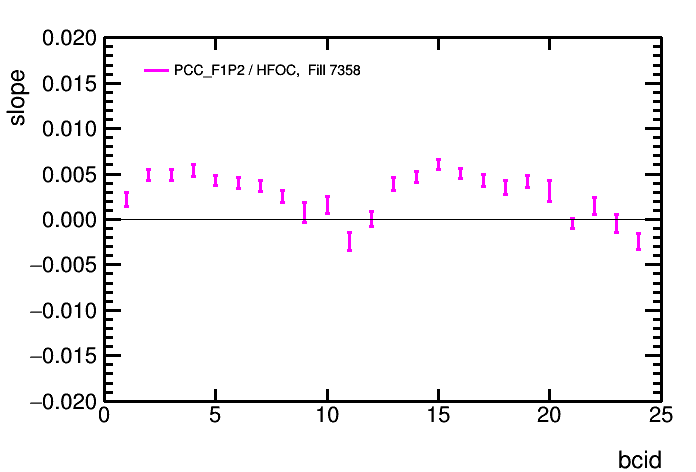
\includegraphics[width=0.32\linewidth]{plots/sbilratios_trains_Fill7358/plot_det_linearity_perbx_slope_7358_F1p2.png}
    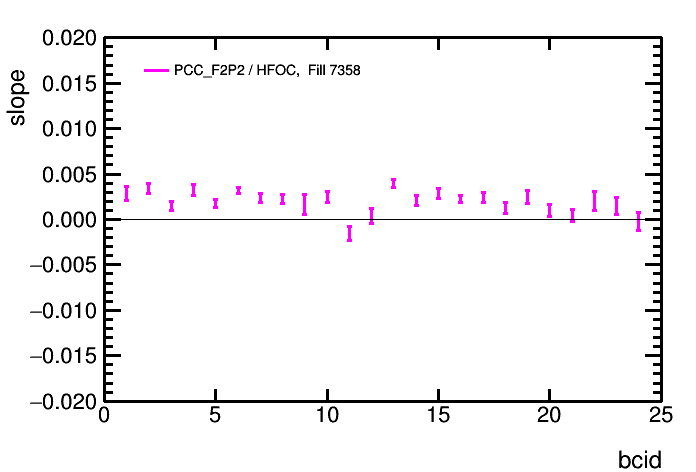
\includegraphics[width=0.32\linewidth]{plots/sbilratios_trains_Fill7358/plot_det_linearity_perbx_slope_7358_F2p2.png}
    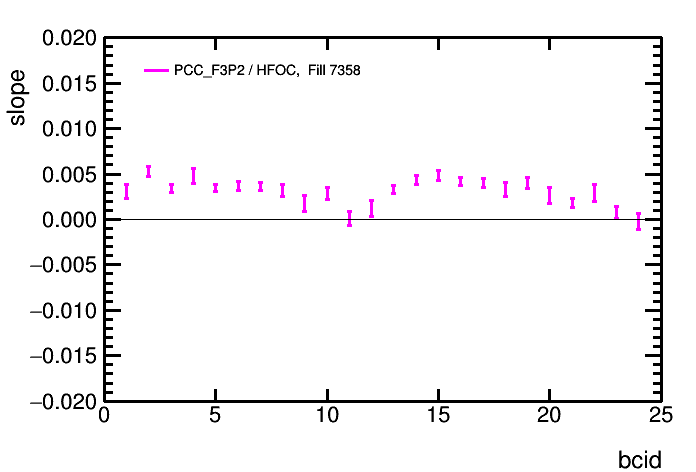
\includegraphics[width=0.32\linewidth]{plots/sbilratios_trains_Fill7358/plot_det_linearity_perbx_slope_7358_F3p2.png}
    \caption{
      Slope values obtained from the linearity fits for the 24 bunches in the two trains of Fill 7358.
      In this plots PCC is shown separately for: \\
      {\bf BPIX} layer 1 (top-left), layer 2 (top-middle), layer 3 (top-right) , \\
      {\bf FPIX Panel 1}:  disk 1 (middle-left), disk 2 (middle-middle), disk 3 (middle-right), and \\
      {\bf FPIX Panel 2}: disk 1 (bottom-left), disk 2 (bottom-middle), disk 3 (bottom-right).
      \label{fig:fill7358trainslope_pccparts}
    }
  \end{center}
\end{figure}

\clearpage
\newpage
\section{Summary}
In this note the relative linearity between PCC and other luminometers has been studied using special runs recorded in 2018 which included pileup scans up to 100.
The linearity is determined by fitting the ratio of two luminometers as a funcion of SBIL measured by a reference detector, in this case the HFOC has been chosen as reference.
Isolated, leading, and train bunches are used to study the variations and train or afterglow effects.

Using isolated and leading bunches a slope of $0.32\pm0.04 \% [Hz/\mu b]^{-1}$ is obtained for the PCC/HFOC comparison.
For train bunches in fill 7358 a systematic decrease is observed in the slope as a function of the bunch id, where the slope becomes negative after 12 bunches.
This effect has been studied by removing the afterglow corrections for PCC and HFOC and by dividing the PCC into subdetectors.
This effect indicates the PCC suffers a loss in cluster counts possibly due to high occupancies at high pileup. 
A variation of the effect is observed for different parts of the Pixel detector.



% >> acknowledgments (for journal papers only)
% The latest version of the acknowledgments will be included from https://twiki.cern.ch/twiki/bin/viewauth/CMS/Internal/PubAcknow as of the date of submission. Modify to match either US or UK English spelling for centre/center, programme/program. For PRL use the short version, for JINST normally use the long version. All others take the middle length version other than exceptional cases.
%\begin{acknowledgments}
%\end{acknowledgments}

%% **DO NOT REMOVE BIBLIOGRAPHY**
\bibliography{auto_generated}   % will be created by the tdr script.

%% examples of appendices.
\clearpage
\appendix
\section{Pixel module veto list}
\label{sec:appendix1}
%!TEX root = ../thesis.tex
% ******************************* Thesis Appendix A ****************************
\chapter{Values for \protect \texorpdfstring{$\alpha$ and $\mu$}{and}}
\begin{verbatim}
Floating Parameter		\qquad		FinalValue +/- Error \\
$---------------------------------$			\\
Lumi \quad	\qquad	\qquad		\qquad		1.0082e+00 +/-  2.42e-02\\
alpha\_sample\_tth\_sys	\quad	1.9100e-01 +/-  9.94e-01\\
alpha\_sample\_ttw\_sys	\quad	8.7537e-01 +/-  9.18e-01\\
alpha\_sample\_ttz\_sys	\quad	2.0012e-01 +/-  9.95e-01\\
alpha\_sample\_tz\_sys\qquad	1.6749e-01 +/-  1.00e+00\\
alpha\_sample\_wz\_sys\qquad	 1.2732e-01 +/-  9.84e-01 \\
alpha\_sample\_fakes\_sys	4.5030e-01 +/-  7.17e-01\\
mu 	\qquad	\qquad	\qquad	\qquad	\qquad	2.4975e+00 +/-  1.29e+01
\end{verbatim}


\begin{verbatim}
Floating Parameter			\qquad		FinalValue +/- Error \\
$-----------------------------$
Lumi \quad	\qquad	\qquad		\qquad	\qquad 1.0085e+00 +/-  2.40e-02\\
alpha\_sample\_tth\_sys	\quad	1.9290e-01 +/-  1.00e+00 \\
alpha\_sample\_ttw\_sys	\quad	8.7911e-01 +/-  9.42e-01\\
alpha\_sample\_ttz\_sys	\quad	2.0370e-01 +/-  9.94e-01\\
alpha\_sample\_tz\_sys\qquad	1.8269e-01 +/-  9.69e-01\\
alpha\_sample\_wz\_sys\qquad	1.4244e-01 +/-  9.99e-01\\
alpha\_sample\_fakes\_sys	1.4243e-01 +/-  9.98e-01\\
mu \qquad	\qquad	\qquad	\qquad	\qquad 6.9361e-02 +/-  1.02e+00
\end{verbatim}
\section{Train effect crosscheck}
\label{sec:appendix2}

Two cross-checks have been performed for Fill 7358 to understand if the systematic change in the slope values as a function of bcid are due to the afterglow corrections.
In the first check (Fig~\ref{fig:fill7358trainslope_crosscheckPCC}) the PCC afterglow corrections are removed, in the second check (Fig~\ref{fig:fill7358trainslope_crosscheckHFOC}) the HFOC residual afterglow corrections are removed.
In both tests the y-intercept values change, but the systematic trend on the slope values remains.

\vspace{36pt}
\begin{figure}[hc]
  \begin{center}
    \includegraphics[width=0.47\linewidth]{plots/sbilratios_trains_Fill7358/plot_det_linearity_perbx_y0_7358_NoPCCCorr.png}
    \includegraphics[width=0.47\linewidth]{plots/sbilratios_trains_Fill7358/plot_det_linearity_perbx_slope_7358_NoPCCCorr.png}
    \caption{
      y-intercept and slope values obtained from the linearity fits for the 24 bunches in the two trains of Fill 7358 after removing the PCC afterglow corrections.
      \label{fig:fill7358trainslope_crosscheckPCC}
    }

    \includegraphics[width=0.47\linewidth]{plots/sbilratios_trains_Fill7358/plot_det_linearity_perbx_y0_7358_NoHFCorr.png}
    \includegraphics[width=0.47\linewidth]{plots/sbilratios_trains_Fill7358/plot_det_linearity_perbx_slope_7358_NoHFCorr.png}
    \caption{
      y-intercept and slope values obtained from the linearity fits for the 24 bunches in the two trains of Fill 7358 after removing the HFOC residual afterglow corrections.
      \label{fig:fill7358trainslope_crosscheckHFOC}
    }

  \end{center}
\end{figure}


%\begin{figure}[hb]
%  \begin{center}
%  \end{center}
%\end{figure}
%


%%% DO NOT ADD \end{document}!

